\documentclass{standalone}
\usepackage{tikz}
\usepackage{standalone}
\begin{document}
	
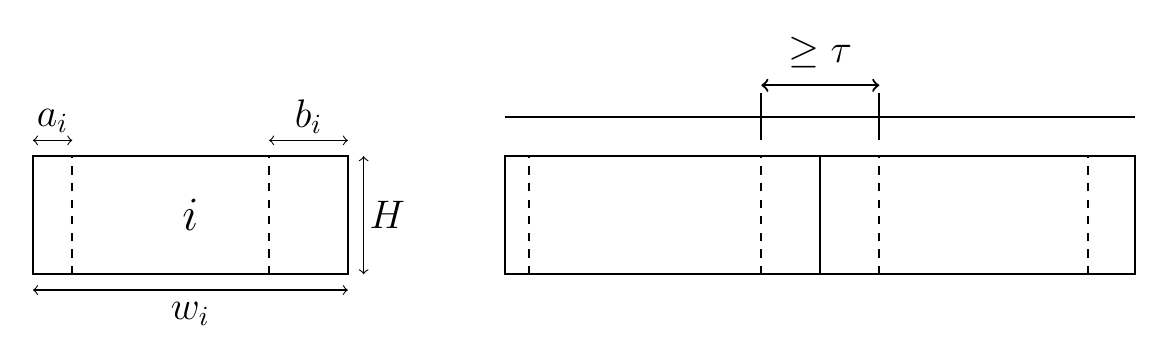
\begin{tikzpicture}
%\draw [help lines] (-2,-2) grid (15,5);

\draw [thick] (0,0) rectangle (4,1.5);
\draw [thick, dashed] (0.5,0) -- (0.5, 1.5);
\draw [thick, dashed] (3,0) -- (3, 1.5);

\draw [<->] (0,-.2) -- (4,-.2);
\node at (2, -.5) {\Large{$w_i$}};

\draw [<->] (0, 1.7) -- (0.5, 1.7);
\node at (0.25, 1.95) {\Large{$a_i$}};

\draw [<->] (3, 1.7) -- (4, 1.7);
\node at (3.5, 2) {\Large{$b_i$}};

\draw [<->] (4.2,0) -- (4.2,1.5);
\node at (4.5,0.75) {\Large{$H$}};

\node at (2,0.75) {\LARGE{$i$}};


\draw [thick] (6,2) -- (14,2);
\draw [thick] (9.25,2.3) -- (9.25,1.7);
\draw [thick] (10.75,2.3) -- (10.75,1.7);
\draw [thick, <->] (9.25, 2.4) -- (10.75, 2.4);
\node [above] at (10,2.5) {\Large{$\geq \tau$}};


\draw [thick] (6,0) rectangle (14,1.5);
\draw [thick] (10,1.5) -- (10,0);
\draw [thick, dashed] (6.3,0) -- (6.3,1.5);
\draw [thick, dashed] (9.25,0) -- (9.25,1.5);
\draw [thick, dashed] (10.75,0) -- (10.75,1.5);
\draw [thick, dashed] (13.4,0) -- (13.4,1.5);

%\draw [<->] (3.5,2.2) -- (4.5,2.2);
%\node at (4, -.4) {\scriptsize $\geq \tau$};







\end{tikzpicture}
	
\end{document}